\chapter{طراحی و پیاده سازی}\label{chapter3}

در این بخش ابتدا پروژه به طور کلی شرح داده شده و در ادامه طراحی بستر بدون سرور اینترنت اشیاء به صورت میکروسرویس توضیح داده می‌شود. پس از معرفی ابزارها و تکنولوژی‌های استفاده شده، نحوه پیاده‌سازی این بستر مورد بررسی قرار می‌گیرد.

\section{دید کلی}

بستر های اینترنت اشیاء بسته به کاربرد، نوع دستگاه‌ها و محیط مورد استفاده با قابلیت‌های مختلفی طراحی می‌شوند. به عنوان مثال یک بستر خانه هوشمند با یک بستر حمل و نقل هوشمند می‌تواند تفاوت‌های زیادی در معماری، نحوه ذخیره سازی، مدیریت و نمایش داده‌ها داشته باشد اما در بسیاری از موارد یکسان هستند. برخی از این موارد عبارتند از:
\begin{itemize}
	
	\item جمع‌‌آوری و ذخیره سازی داده‌های حسگر‌ها به صورت سری زمانی
	
	\item کنترل دستگاه‌ها و ارسال فرمان به آن‌ها
	
	\item مدیریت دستگاه‌ها و کاربران
	
	\item برخورد مناسب با رویداد‌ها
	
	\item پردازش و تحلیل داده‌ها
	
\end{itemize}

مهم‌ترین قابلیت یک بستر اینترنت اشیاء جمع آوری و ذخیره سازی داده‌های حسگر‌ها می‌باشد. این داده‌ها معمولاً به صورت یک پیام با پروتکل \lr{MQTT} به یک \lr{message broker} ارسال می‌شود، پس از احراز هویت دستگاه، به هسته بستر ارسال شده و برای پردازش‌های لازم مورد استفاده قرار می‌گیرد. این پیام همچنین به پایگاه داده فرستاده شده و به صورت سری زمانی ذخیره می‌گردد. سپس این داده‌ها می‌توانند توسط بخش‌های دیگر بستر استخراج و برای تحلیل و مصورسازی به سرویس‌گیرنده ارسال شود. در این پروژه این قابلیت با استفاده از بستر بدون سرور \lr{OpenWhisk} و هماهنگ کننده ابری ‌کوبرنتیز طراحی و پیاده سازی شده است.

\newpage

\section{طراحی}

طراحی این پروژه از چهار بخش اصلی تشکیل شده است. اولین بخش طراحی معماری میکروسرویس \lr{message broker} برای دریافت و ارسال داده‌های حسگر، پایگاه داده برای ذخیره سازی داده‌های سری زمانی و یک پایگاه داده دیگر برای ذخیره سازی \lr{trigger} است. بخش دوم طراحی یک ماژول سرویس‌دهنده به اسم \lr{MQTT trigger provider} است که پیام را از ‌\lr{message broker} دریافت کرده آن را از طریق سیستم \lr{trigger} و \lr{rule} به بستر بدون سرور ارسال می‌کند. بخش سوم شامل طراحی \lr{action} در بستر بدون سرور \lr{OpenWhisk} برای ذخیره سازی و استخراج داده‌های سری زمانی است. در بخش چهارم طراحی یک برنامه کاربردی با استفاده از این بستر در دو بخش سرویس‌دهنده برای ارائه‌ی سرویس‌های دلخواه و بخش سرویس‌گیرنده برای نمایش داده‌ها بررسی می‌شود.
\newline

نمای کلی معماری پروژه در شکل \ref{platformArchitecture} نشان داده شده است.
\newline

\begin{figure}[!h]
	\centering
	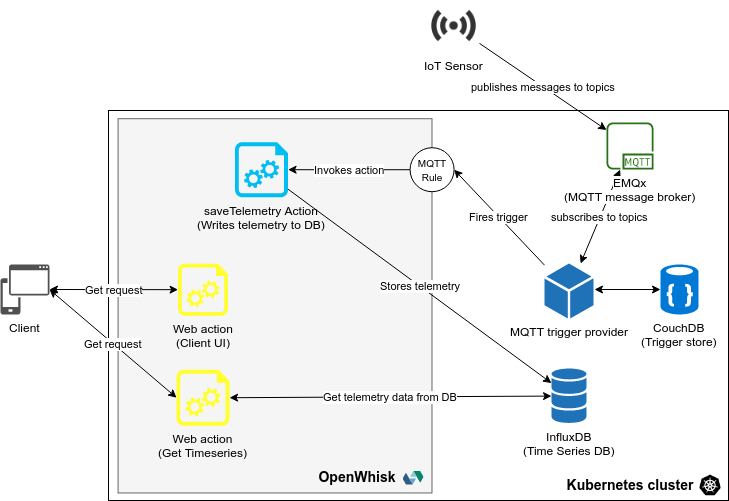
\includegraphics[height=11cm]{images/platform-architecture-1}
	\caption{نمای کلی معماری پروژه}
	\label{platformArchitecture}
\end{figure}

\subsection{طراحی میکروسرویس}

این بستر به صورت میکروسرویس طراحی شده است و عملکردهای مختلف این بستر توسط این میکروسرویس‌ها انجام می‌شوند. در ادامه طراحی معماری این میکروسرویس‌ها را بررسی می‌کنیم:

\begin{itemize}
	
	\item \textbf{\lr{message broker}:} این سرویس برای اتصال دستگاه‌های اینترنت اشیاء به بستر طراحی شده است و پیام‌های ارسالی از طرف دستگاه‌ها را باید به سرویس‌های دیگر بستر که مشترک شده‌اند بفرستد. بنابراین نیاز است که این سرویس از بیرون و درون بستر قابل دسترسی باشد. برای دسترسی از بیرون از قابلیت \lr{expose} کردن \lr{port} توسط کوبرنتیز استفاده شده است. همچنین یک سرویس کوبرنتیز برای اتصال به دیگر سرویس‌های درونی بستر طراحی شده است.
	
	\item \textbf{\lr{trigger store}:} این سرویس یک پایگاه داده \lr{CouchDB} است که باید \lr{trigger} ها را ذخیره کند. دسترسی و اتصال به این سرویس از داخل بستر پس از راه‌اندازی به راحتی امکان پذیر است و تنها نیاز به تنظیم کردن و مهیا نمودن پایگاه داده برای ذخیره و بازیابی داده‌های مورد نیاز است. 
	
	\item \textbf{\lr{timeseries database}:} پایگاه داده سری زمانی \lr{InfluxDB} است. این پایگاه داده برای ذخیره‌سازی داده‌های سری زمانی دستگاه‌ها طراحی شده است و پس از راه‌اندازی توسط سرویس‌های دیگر درون بستر در دسترس است.
	
	\item \textbf{\lr{OpenWhisk}:} پیاده‌سازی و راه‌اندازی بستر \lr{OpenWhisk} بر روی بستر کوبرنتیز توسط یک پروژه که به همین منظور طراحی شده است، وجود دارد. این پروژه، اجزای \lr{OpenWhisk} را به صورت اشیاء کوبرنتیز درون یک \lr{namespace} جدا راه‌اندازی می‌کند. سرویس‌هایی طراحی شده است که ارتباط این بستر را با سرویس‌های دیگر درون \lr{namespace} اصلی برقرار می‌سازد.
	
\end{itemize}

\subsection{\lr{MQTT trigger provider}}

این قسمت از بستر برای اشتراک و دریافت پیام از  \lr{message broker} و ارسال آن به بستر بدون سرور برای ذخیره سازی طراحی شده است. با افزوده شدن یک \lr{trigger} در بستر بدون سرور برای دریافت پیام ها بر روی یک \lr{topic} جدید، این سرویس آن را دریافت می‌کند و بر روی آن \lr{topic} مشترک می‌شود. همچنین \lr{trigger} ها را در یک پایگاه داده ذخیره می‌کند تا در هنگام راه‌اندازی مجدد سرویس بتواند  دوباره بر روی آن \lr{topic} ها مشترک شود.

\subsection{مدیریت داده‌های سری زمانی}

پس از شلیک شدن \lr{trigger} توسط سرویس \lr{MQTT trigger provider}، پیام باید پردازش و داده موجود در آن در پایگاه داده ذخیره شود. یک \lr{action} با نام \lr{saveTelemetry} برای این کار طراحی شده‌ است و \lr{trigger} شلیک شده با تعریف کردن یک \lr{rule} به آن متصل می‌شود. این \lr{action} یک تابع است که با دریافت پیام آن را باز کرده و با فرمت مشخص برای ذخیره سازی به پایگاه داده سری زمانی می‌فرستد.

برای استخراج داده‌های سری زمانی از پایگاه داده یک \lr{action} دیگر به اسم \lr{getTimeseries} طراحی شده است که با گرفتن \lr{token} دستگاه و کلید‌های داده‌ها، داده‌های مشخص شده با کلید و مربوط به آن دستگاه را به صورت سری زمانی برمی‌گرداند. این \lr{action} همچنین پارامتر دیگری به نام \lr{limit} برای محدود کردن تعداد داده‌های سری زمانی دارد و اگر برابر \lr{n} باشد به این معنی است که \lr{n} تا از آخرین داده‌ها در پاسخ ارسال شوند. در صورتی که این پارامتر وجود نداشته باشد تنها آخرین داده ارسال خواهد شد. برای این \lr{action} دسترسی وب نیز تعریف می‌شود تا بتوان آن را از طریق درخواست \lr{HTTP} اجرا کرد.

\subsection{برنامه کاربردی}

تا اینجا طراحی بستر به پایان رسید. پس از ایجاد \lr{trigger} با \lr{topic} مشخص، دستگاه می‌تواند داده‌های خود را در قالب پیام‌های \lr{MQTT} به \lr{broker} ارسال کند و این داده‌ها در پایگاه داده ذخیره شده و در دسترس خواهند بود. حال کاربران می‌توانند به توسعه برنامه کاربردی خود بپردازند. با تعریف تابع‌ها در قالب \lr{action} می‌توان از داده‌های سری زمانی ذخیره شده برای پردازش‌های مختلف استفاده کرد. با تعریف کردن \lr{rule} می‌توان سناریوهای دلخواهی تعریف کرد که در هنگام دریافت پیام یا شلیک \lr{trigger} تعریف شده اجرا شوند. همچنین معماری \lr{RESTful APIs} نیز با تعریف کردن \lr{action} ها به عنوان \lr{web action} به سادگی امکان پذیر است.

حال برای نمونه یک برنامه‌ی کاربردی با استفاده از \lr{action} ها طراحی شده است. این برنامه در ابتدا دستگاه‌های موجود را گرفته و نمایش می‌دهد و پس از انتخاب هر دستگاه، داده‌های ارسالی توسط آن دستگاه به صورت بلادرنگ نمایش داده می‌شود.

\newpage

\section{تکنولوژی‌های استفاده شده}

\subsection{\lr{MicroK8s}}

\lr{MicroK8s} این امکان را فراهم می‌سازد تا با اجرای یک دستور، یک نود کوبرنتیز برای ایجاد یک محیط توسعه و تست به صورت محلی نصب و اجرا شود. نصب و اجرای \lr{MicroK8s} بسیار سریع و آسان است و بسیاری از بسته‌های مورد نیاز برای توسعه‌ی محلی برنامه‌های کاربردی را شامل می‌شود. از آن جایی که راه‌اندازی کوبرنتیز کمی تخصصی و پیچیده است و همچنین بسته‌های مورد نیاز دیگری باید به صورت دستی بر روی آن نصب شود، استفاده از یک ابزار که تمامی این کارها را به صورت خودکار انجام می‌دهد بسیار مفید است \cite{microk8s}.

ابزار دیگری به نام \lr{MiniKube} وجود دارد که یک نود کوبرنتیز را بر روی یک ماشین مجازی درون سیستم عامل راه‌اندازی می‌کند. این ابزار نیز مخصوص توسعه و تست است. این ابزار بر روی تمامی سیستم عامل‌ها قابل اجرا است، اما \lr{MicroK8s} فقط از سیستم عامل لینوکس\LTRfootnote{Linux} پشتیبانی می‌کند \cite{minikube}.

\subsection{\lr{Helm}}

ابزار مدیریت پکیج‌هایی است که برای پیاده‌سازی بر روی بستر کوبرنتیز تنظیم شده‌اند. این منابع از پیش تنظیم شده با نام \lr{charts} شناخته می‌شوند. با کمک \lr{Helm} می‌توان پکیج‌ها و منابعی که به صورت شخصی ساخته می‌شود را به اشتراک گذاشت. همچنین امکان به‌روز رسانی محصولات توسط این ابزار وجود دارد \cite{helm}.

\subsection{\lr{EMQx}}

\lr{EMQx} یک \lr{message broker} توزیع شده با پروتکل \lr{MQTT} برای اینترنت اشیاء، ارتباط ماشین به ماشین\LTRfootnote{M2M} و برنامه‌های کاربردی تلفن همراه است؛ کاملاً متن باز، بسیار مقیاس‌پذیر و بسیار در دسترس است که یک خوشه آن می تواند ده‌ها میلیون سرویس‌گیرنده را همزمان اداره کند. بیش از ۵ هزار شرکت از این \lr{message boker} برای اتصال به ۵۰ میلیون دستگاه اینترنت اشیاء استفاده می‌کنند \cite{emqx}.

\subsection{\lr{CouchDB}}

\lr{CouchDB} یک پایگاه داده \lr{NoSQL}، سند محور و متن باز است که با زبان همگام \lr{Erlang} پیاده‌سازی شده است. از \lr{JSON} برای ذخیره داده ها، از زبان \lr{JavaScript‌} به عنوان زبان اجرای دستور و از ‌\lr{HTTP} برای \lr{API} استفاده می‌کند.

برخلاف یک پایگاه داده رابطه‌ای\LTRfootnote{relational database}، پایگاه داده \lr{CouchDB} داده‌ها و روابط را در جدول‌ها ذخیره نمی‌کند. در عوض، هر بانک اطلاعاتی مجموعه ای از اسناد مستقل است. ویژگی متمایز کننده‌ی \lr{CouchDB} همانند‌سازی ‌مولتی-مستر\LTRfootnote{multi-master replication} است که به آن اجازه می‌دهد تا در دستگاه‌ها مقیاس شود و سیستم‌های با کارایی بالا بسازد \cite{couchdb}.

\subsection{\lr{InfluxDB}}

\lr{InfluxDB} یک پایگاه داده سری زمانی\LTRfootnote{Time Series Data Base (TSDB)} متن باز است که توسط شرکت \lr{InfluxData} و با زبان \lr{Go} نوشته شده است. همچنین برای ذخیره‌سازی سریع، در دسترس بودن بالا و بازیابی داده‌های سری زمانی در زمینه هایی مانند نظارت بر عملیات، اندازه‌گیری برنامه‌ها، داده‌های حسگرهای اینترنت اشیاء و تجزیه و تحلیل بلادرنگ بهینه شده است. این پایگاه داده از زبان شبیه به \lr{SQL} برای اجرای دستورات استفاده می‌کند \cite{influxdb}.

\newpage

\section{پیاده سازی}

حال پس از بررسی طراحی و آشنایی با تکنولوژی‌های مورد نیاز به پیاده سازی این بستر می‌پردازیم. اولین مرحله‌ی پیاده سازی، فراهم نمودن یک خوشه از هماهنگ کننده ابری کوبرنتیز است. این هماهنگ کننده می‌تواند از سرویس‌ ارائه دهندگان ابری تهیه شده یا به صورت دستی روی سرور‌های خصوصی ‌پیاده سازی شود. برای پیاده سازی محلی نیز می‌توان از برنامه‌ی \lr{minikube} استفاده کرد. این برنامه یک ماشین مجازی به صورت محلی می‌سازد و کوبرنتیز را درون آن ماشین مجازی پیاده سازی و اجرا می‌کند. در این پروژه از \lr{MicroK8s} برای این منظور استفاده شده است.

پس از اجرای هماهنگ کننده ابری نوبت به پیاده‌سازی سایر میکروسرویس‌ها می‌رسد. برای راه اندازی میکروسرویس‌ها ابتدا باید تنظیم کننده‌ی بسته \lr{Helm} نصب و راه اندازی شود. سپس با استفاده از \lr{Helm} بسته‌های \lr{EMQx}، پایگاه داده ‌\lr{CouchDB} و پایگاه داده سری زمانی \lr{InfluxDB} از طریق \lr{chart} هایشان نصب و اجرا می‌شوند. هر میکروسرویس پس از اجرا باید تنظیمات مورد نیازش انجام شود و برای اطمینان از صحت عملکرد مورد تست قرار گیرد.

\subsection{\lr{OpenWhisk}}

پیاده سازی \lr{OpenWhisk} نیز توسط \lr{Helm} انجام می‌شود. ابتدا باید پروژه‌ای که به همین منظور ساخته شده است را متناسب با نحوه‌ی پیاده‌سازی تنظیم کرده و مورد استفاده قرار داد. این تنظیمات عبارتند از فعال سازی یک نود \lr{ingress} و تعریف کردن \lr{host name} و \lr{port} برای ایجاد راه دسترسی به \lr{OpenWhisk}. این نود با اتصال به \lr{NginX}  درون \lr{OpenWhisk} ارتباط با این بستر را از طریق وب میسر می‌سازد. همچنین تنظیمات دیگری برای نحوه‌ی ذخیره سازی داده‌های پایگاه داده \lr{CouchDB} توسط کوبرنتیز امکان‌پذیر است. در انتها این تنظیمات درون یک فایل ذخیره شده و \lr{OpenWhisk} با اجرای یک دستور \lr{CLI} در یک \lr{namespace} جدا راه اندازی می‌شود.

\subsection{\lr{MQTT trigger provider}}

این ماژول برای راه اندازی در بستر کوبرنتیز باید به صورت کانتینر در بیاید. بنابراین یک فایل داکر برای ساخت کانتینر نوشته شده است. ایمیج این کانتینر توسط این فایل ساخته شده و در \lr{Docker Hub} آپلود می‌شود. پس از آن فایلی برای تعریف یک \lr{deployment} نوشته می‌شود تا این کانتینر را در بستر کوبرنتیز راه اندازی کند. در این فایل پس از مشخص کردن اطلاعات ایمیج کانتینر و \lr{deployment} باید \lr{port} کانتینر و متغیرهای محیطی لازم برای اتصال به سایر سرویس‌ها مشخص شود. این متغیرها عبارتند از نام کاربری، رمزعبور، آدرس و \lr{port} مورد نیاز برای اتصال به پایگاه داده \lr{CouchDB} و همچنین آدرس سرویس \lr{OpenWhisk}. اطلاعات رمزعبور و نام کاربری از طریق \lr{secret} کوبرنتیز در دسترس هستند. فایل تنظیمات \lr{deployment} در شکل \ref{deployment-yml} نشان داده شده است.

\begin{figure}[!h]
	\centering
	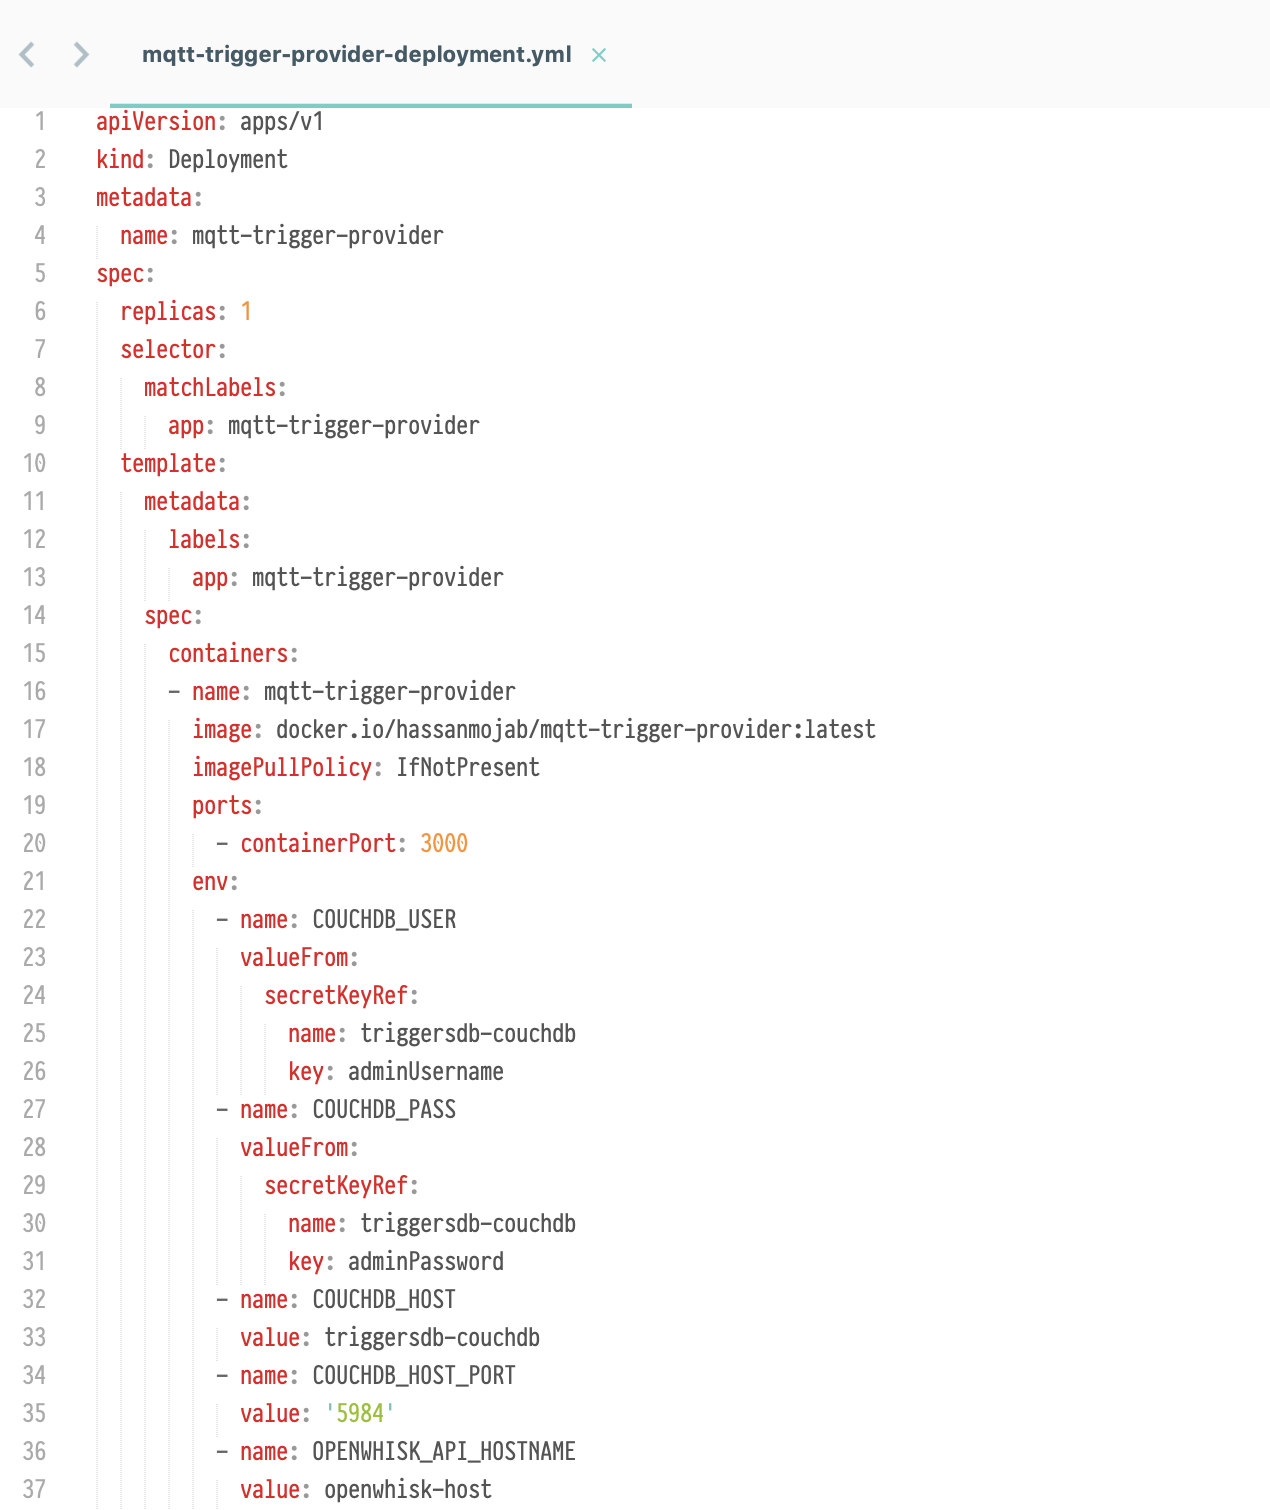
\includegraphics[height=18cm]{images/deployment-yml}
	\caption{سرویس‌های بستر بدون سرور اینترنت اشیاء}
	\label{deployment-yml}
\end{figure}

\subsection{سرویس‌های کوبرنتیز}

برای متصل شدن بقیه اجزاء با یکدیگر باید سرویس‌های دیگری تعریف شود. این سرویس‌ها در قالب فایل‌های مجزا تعریف شده و در انتها با اجرای یک دستور \lr{CLI} توسط کوبرنتیز خوانده و اعمال می‌شوند. این سرویس‌ها عبارتند از:

\begin{itemize}

	\item سرویس \lr{cluster IP} برای اتصال \lr{EMQx} و \lr{OpenWhisk} به \lr{MQTT trigger provider}
	
	\item سرویس \lr{cluster IP} برای اتصال به \lr{OpenWhisk NginX}
	
	\item سرویس \lr{external name} برای اتصال به سرویس \lr{OpenWhisk} از \lr{namespace} اصلی
	
	\item سرویس \lr{external name} برای اتصال به سرویس \lr{MQTT trigger provider} از \lr{namespace} مربوط به \lr{OpenWhisk}
	
	\item سرویس \lr{external name} برای اتصال به سرویس پایگاه داده \lr{InfluxDB} از \lr{namespace} مربوط به \lr{OpenWhisk}

\end{itemize}

پس از اعمال، سرویس‌های در حال اجرا توسط دستور \lr{CLI} قابل مشاهده هستند. سرویس‌های در حال اجرای این بستر در \lr{namespce} های \lr{default} و \lr{openwhisk} در شکل \ref{kubectl-svc} نشان داده شده است.

\begin{figure}[!h]
	\centering
	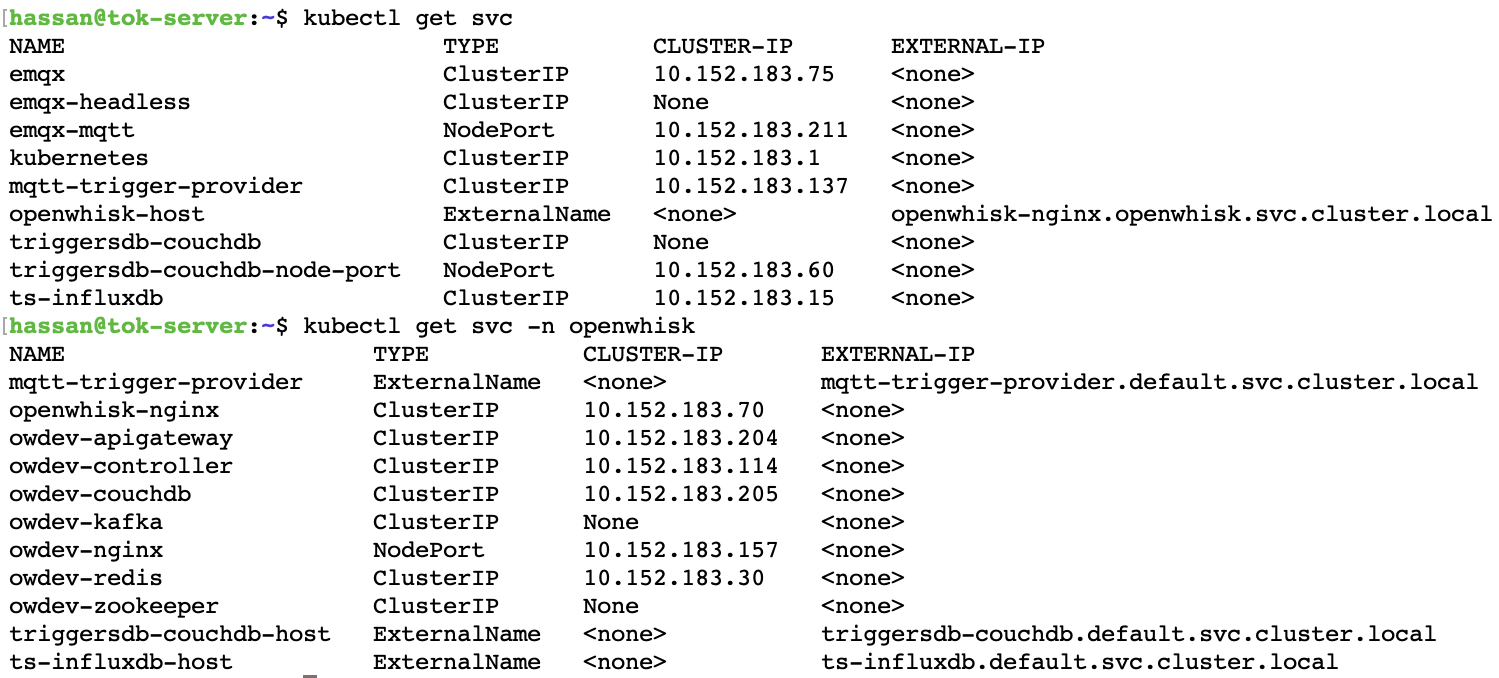
\includegraphics[height=7cm]{images/kubectl-svc}
	\caption{سرویس‌های بستر بدون سرور اینترنت اشیاء}
	\label{kubectl-svc}
\end{figure}

\subsection{\lr{action} ها و \lr{trigger} ها}

برای پیاده سازی \lr{action} ها و \lr{trigger} ها در \lr{OpenWhisk} از رابط \lr{CLI} آن استفاده می‌شود. ابتدا باید \lr{feed action} طراحی شده برای ایجاد و حذف \lr{trigger} ها در \lr{MQTT trigger provider} راه اندازی شود. بنابراین توسط کاربر ادمین \lr{OpenWhisk} یک \lr{package} به نام \lr{mqtt} ساخته شده و برای همه‌ی کاربران به اشتراک گذاشته می‌شود. سپس تابع \lr{feed action} درون این \lr{package} آپلود می‌شود.

حال کاربر می‌تواند یک \lr{trigger} با \lr{feed} تعریف شده برای یک \lr{topic} مشخص، راه اندازی کند و پس از آن تابع \lr{saveTelemetry} را به عنوان \lr{action} آپلود کند. در انتها با تعریف کردن یک \lr{rule} اتصال \lr{trigger} به این \lr{action} برقرار می‌شود. اجرای دستورات تمامی این مراحل در شکل \ref{wsk} قابل مشاهده است.

\begin{figure}[!h]
	\centering
	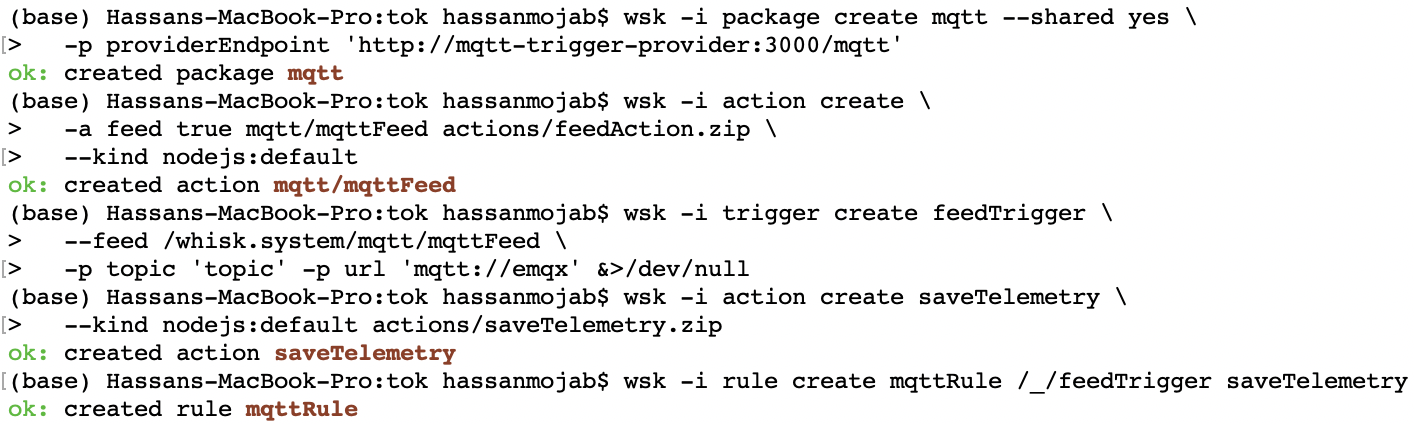
\includegraphics[height=5cm]{images/wsk}
	\caption{ساخت \lr{feed action}، \lr{trigger} و \lr{rule}}
	\label{wsk}
\end{figure}

تابع طراحی شده برای دریافت داده‌های سری زمانی نیز به عنوان یک \lr{web action} آپلود شده و توسط یک دستور \lr{CLI} می‌توان آدرس آن را در قالب \lr{URL} دریافت کرد (شکل \ref{wsk-action}).

\begin{figure}[!h]
	\centering
	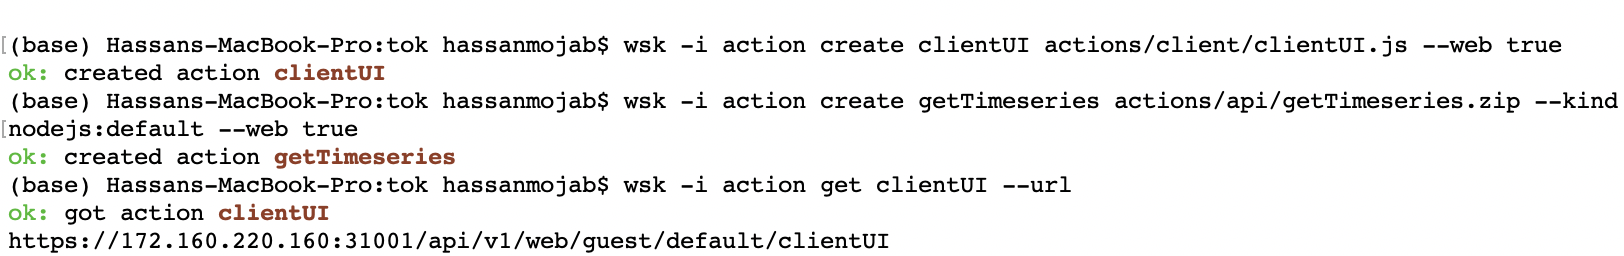
\includegraphics[height=2.7cm]{images/wsk-action}
	\caption{آپلود \lr{web action} و دریافت آدرس آن}
	\label{wsk-action}
\end{figure}

پیاده‌سازی بستر تا اینجا به اتمام می‌رسد اما توسعه‌ی برنامه‌های کاربردی مختلف و دلخواه بر روی این بستر توسط کاربران امکان‌پذیر است. توسعه‌ی این برنامه‌ها در سطح تابع است و مراحل آن عبارت است از تعریف کردن تابع ها به عنوان \lr{action} های \lr{OpenWhisk}، استفاده از قابلیت زنجیر کردن \lr{action} ها، استفاده از سیستم \lr{rule} و \lr{trigger} برای ساخت سناریوها و قابلیت‌های دیگر بستر که قبلاً توضیح داده شد.
